% Options for packages loaded elsewhere
\PassOptionsToPackage{unicode}{hyperref}
\PassOptionsToPackage{hyphens}{url}
\PassOptionsToPackage{dvipsnames,svgnames,x11names}{xcolor}
%
\documentclass[
  10pt,
  ignorenonframetext,
]{beamer}
\usepackage{pgfpages}
\setbeamertemplate{caption}[numbered]
\setbeamertemplate{caption label separator}{: }
\setbeamercolor{caption name}{fg=normal text.fg}
\beamertemplatenavigationsymbolsempty
% Prevent slide breaks in the middle of a paragraph
\widowpenalties 1 10000
\raggedbottom
\setbeamertemplate{part page}{
  \centering
  \begin{beamercolorbox}[sep=16pt,center]{part title}
    \usebeamerfont{part title}\insertpart\par
  \end{beamercolorbox}
}
\setbeamertemplate{section page}{
  \centering
  \begin{beamercolorbox}[sep=12pt,center]{part title}
    \usebeamerfont{section title}\insertsection\par
  \end{beamercolorbox}
}
\setbeamertemplate{subsection page}{
  \centering
  \begin{beamercolorbox}[sep=8pt,center]{part title}
    \usebeamerfont{subsection title}\insertsubsection\par
  \end{beamercolorbox}
}
\AtBeginPart{
  \frame{\partpage}
}
\AtBeginSection{
  \ifbibliography
  \else
    \frame{\sectionpage}
  \fi
}
\AtBeginSubsection{
  \frame{\subsectionpage}
}
\usepackage{amsmath,amssymb}
\usepackage{lmodern}
\usepackage{setspace}
\usepackage{iftex}
\ifPDFTeX
  \usepackage[T1]{fontenc}
  \usepackage[utf8]{inputenc}
  \usepackage{textcomp} % provide euro and other symbols
\else % if luatex or xetex
  \usepackage{unicode-math}
  \defaultfontfeatures{Scale=MatchLowercase}
  \defaultfontfeatures[\rmfamily]{Ligatures=TeX,Scale=1}
\fi
% Use upquote if available, for straight quotes in verbatim environments
\IfFileExists{upquote.sty}{\usepackage{upquote}}{}
\IfFileExists{microtype.sty}{% use microtype if available
  \usepackage[]{microtype}
  \UseMicrotypeSet[protrusion]{basicmath} % disable protrusion for tt fonts
}{}
\makeatletter
\@ifundefined{KOMAClassName}{% if non-KOMA class
  \IfFileExists{parskip.sty}{%
    \usepackage{parskip}
  }{% else
    \setlength{\parindent}{0pt}
    \setlength{\parskip}{6pt plus 2pt minus 1pt}}
}{% if KOMA class
  \KOMAoptions{parskip=half}}
\makeatother
\usepackage{xcolor}
\geometry{left = 1cm, right = 0.5cm, top = 0.5cm, bottom = 0.5cm}
\newif\ifbibliography
\usepackage{color}
\usepackage{fancyvrb}
\newcommand{\VerbBar}{|}
\newcommand{\VERB}{\Verb[commandchars=\\\{\}]}
\DefineVerbatimEnvironment{Highlighting}{Verbatim}{commandchars=\\\{\}}
% Add ',fontsize=\small' for more characters per line
\usepackage{framed}
\definecolor{shadecolor}{RGB}{248,248,248}
\newenvironment{Shaded}{\begin{snugshade}}{\end{snugshade}}
\newcommand{\AlertTok}[1]{\textcolor[rgb]{0.94,0.16,0.16}{#1}}
\newcommand{\AnnotationTok}[1]{\textcolor[rgb]{0.56,0.35,0.01}{\textbf{\textit{#1}}}}
\newcommand{\AttributeTok}[1]{\textcolor[rgb]{0.77,0.63,0.00}{#1}}
\newcommand{\BaseNTok}[1]{\textcolor[rgb]{0.00,0.00,0.81}{#1}}
\newcommand{\BuiltInTok}[1]{#1}
\newcommand{\CharTok}[1]{\textcolor[rgb]{0.31,0.60,0.02}{#1}}
\newcommand{\CommentTok}[1]{\textcolor[rgb]{0.56,0.35,0.01}{\textit{#1}}}
\newcommand{\CommentVarTok}[1]{\textcolor[rgb]{0.56,0.35,0.01}{\textbf{\textit{#1}}}}
\newcommand{\ConstantTok}[1]{\textcolor[rgb]{0.00,0.00,0.00}{#1}}
\newcommand{\ControlFlowTok}[1]{\textcolor[rgb]{0.13,0.29,0.53}{\textbf{#1}}}
\newcommand{\DataTypeTok}[1]{\textcolor[rgb]{0.13,0.29,0.53}{#1}}
\newcommand{\DecValTok}[1]{\textcolor[rgb]{0.00,0.00,0.81}{#1}}
\newcommand{\DocumentationTok}[1]{\textcolor[rgb]{0.56,0.35,0.01}{\textbf{\textit{#1}}}}
\newcommand{\ErrorTok}[1]{\textcolor[rgb]{0.64,0.00,0.00}{\textbf{#1}}}
\newcommand{\ExtensionTok}[1]{#1}
\newcommand{\FloatTok}[1]{\textcolor[rgb]{0.00,0.00,0.81}{#1}}
\newcommand{\FunctionTok}[1]{\textcolor[rgb]{0.00,0.00,0.00}{#1}}
\newcommand{\ImportTok}[1]{#1}
\newcommand{\InformationTok}[1]{\textcolor[rgb]{0.56,0.35,0.01}{\textbf{\textit{#1}}}}
\newcommand{\KeywordTok}[1]{\textcolor[rgb]{0.13,0.29,0.53}{\textbf{#1}}}
\newcommand{\NormalTok}[1]{#1}
\newcommand{\OperatorTok}[1]{\textcolor[rgb]{0.81,0.36,0.00}{\textbf{#1}}}
\newcommand{\OtherTok}[1]{\textcolor[rgb]{0.56,0.35,0.01}{#1}}
\newcommand{\PreprocessorTok}[1]{\textcolor[rgb]{0.56,0.35,0.01}{\textit{#1}}}
\newcommand{\RegionMarkerTok}[1]{#1}
\newcommand{\SpecialCharTok}[1]{\textcolor[rgb]{0.00,0.00,0.00}{#1}}
\newcommand{\SpecialStringTok}[1]{\textcolor[rgb]{0.31,0.60,0.02}{#1}}
\newcommand{\StringTok}[1]{\textcolor[rgb]{0.31,0.60,0.02}{#1}}
\newcommand{\VariableTok}[1]{\textcolor[rgb]{0.00,0.00,0.00}{#1}}
\newcommand{\VerbatimStringTok}[1]{\textcolor[rgb]{0.31,0.60,0.02}{#1}}
\newcommand{\WarningTok}[1]{\textcolor[rgb]{0.56,0.35,0.01}{\textbf{\textit{#1}}}}
\setlength{\emergencystretch}{3em} % prevent overfull lines
\providecommand{\tightlist}{%
  \setlength{\itemsep}{0pt}\setlength{\parskip}{0pt}}
\setcounter{secnumdepth}{-\maxdimen} % remove section numbering
\usepackage{float}
\usepackage{booktabs}
\usepackage{array}
\usepackage{multirow}
\usepackage{graphicx}
\setbeamertemplate{itemize item}{$\diamond$}
\setbeamertemplate{itemize subitem}{\scriptsize$\diamond$}
\setbeamertemplate{navigation symbols}{}
\setbeamertemplate{footline}[page number]
\definecolor{blue}{RGB}{0,114,178}
\definecolor{red}{RGB}{213,94,0}
\definecolor{yellow}{RGB}{240,228,66}
\definecolor{green}{RGB}{0,158,115}
\ifLuaTeX
  \usepackage{selnolig}  % disable illegal ligatures
\fi
\IfFileExists{bookmark.sty}{\usepackage{bookmark}}{\usepackage{hyperref}}
\IfFileExists{xurl.sty}{\usepackage{xurl}}{} % add URL line breaks if available
\urlstyle{same} % disable monospaced font for URLs
\hypersetup{
  pdftitle={Econometrics: Multiple Regression and Applications},
  pdfauthor={Duong Trinh},
  colorlinks=true,
  linkcolor={blue},
  filecolor={Maroon},
  citecolor={Blue},
  urlcolor={Blue},
  pdfcreator={LaTeX via pandoc}}

\title{Econometrics: Multiple Regression and Applications}
\subtitle{ECON4004: LAB 2}
\author{Duong Trinh}
\date{February 14, 2024}
\institute{University of Glasgow}

\begin{document}
\frame{\titlepage}

\setstretch{1.5}
\begin{frame}{Intro}
\protect\hypertarget{intro}{}
\begin{itemize}
\tightlist
\item
  Duong Trinh

  \begin{itemize}
  \tightlist
  \item
    PhD Student in Economics (Bayesian Microeconometrics)
  \item
    Email: \underline{Duong.Trinh@glasgow.ac.uk}
  \end{itemize}
\end{itemize}

\vspace{3mm}

\begin{itemize}
\tightlist
\item
  ECON4004-LB01

  \begin{itemize}
  \tightlist
  \item
    Wednesday 10am -12 pm
  \item
    5 sessions (7-Feb, 14-Feb, 21-Feb, 28-Feb, 6-March)
  \item
    ST ANDREWS:357
  \end{itemize}
\item
  ECON4004-LB02

  \begin{itemize}
  \tightlist
  \item
    Wednesday 12-2 pm
  \item
    5 sessions (7-Feb, 14-Feb, 21-Feb, 28-Feb, 6-March)
  \item
    ST ANDREWS:357
  \end{itemize}
\end{itemize}
\end{frame}

\begin{frame}{Record Attendance}
\protect\hypertarget{record-attendance}{}
\end{frame}

\begin{frame}{Plan for LAB 2}
\protect\hypertarget{plan-for-lab-2}{}
\begin{itemize}
\tightlist
\item
  Exercise 2: based on Stock and Watson, E13.1
\item
  Exercise 1: based on Stock and Watson, E8.1
\end{itemize}

\vspace{3mm}

\begin{itemize}
\tightlist
\item
  We will focus on \emph{incorporating interactions between two
  independent variables into a regression model}.
\end{itemize}
\end{frame}

\hypertarget{exercise-2-based-on-stock-and-watson-e13.1}{%
\section{Exercise 2: based on Stock and Watson,
E13.1}\label{exercise-2-based-on-stock-and-watson-e13.1}}

\begin{frame}[fragile]{Picture the Scenario}
\protect\hypertarget{picture-the-scenario}{}
\begin{itemize}
\tightlist
\item
  \textbf{Objective:} Examine Labor Market Discrimination: Are Emily and
  Greg More Employable Than Lakisha and Jamal?
\end{itemize}

\vspace{0.8mm}

\begin{itemize}
\tightlist
\item
  \textbf{Dataset:} \texttt{Names.dta}

  \begin{itemize}
  \tightlist
  \item
    Experimental data from research on US labor market.
  \end{itemize}
\end{itemize}

\vspace{0.8mm}

\begin{itemize}
\tightlist
\item
  \textbf{Key variables:}

  \begin{itemize}
  \tightlist
  \item
    \texttt{call\_back}: callback rate, measured by fraction of resumes
    that generate a phone call from prospective employer.
  \item
    \texttt{black}: \(= 1\) for ``African American--sounding name''
    resumes, \(= 0\) for ``white-sounding name'' resumes.
  \item
    \texttt{female}: \(= 1\) for women, \(= 0\) for men.
  \item
    \texttt{high}: \(= 1\) for high-quality resumes, \(= 0\) for
    low-quality resumes.
  \end{itemize}
\end{itemize}
\end{frame}

\begin{frame}{Picture the Scenario}
\protect\hypertarget{picture-the-scenario-1}{}
Randomized Controlled Experiment
\href{https://pubs-aeaweb-org.ezproxy2.lib.gla.ac.uk/doi/pdfplus/10.1257/0002828042002561}{(Bertrand
and Mullainathan, 2004)}

\begin{itemize}
\item
  A prospective employer receives two resumes: a resume from a white job
  applicant and a similar resume from an African American applicant. Is
  the employer more likely to call back the white applicant to arrange
  an interview?
\item
  Because race is not typically included on a resume, they
  differentiated resumes on the basis of ``white-sounding names'' such
  as Emily Walsh or Gregory Baker) and ``African American--sounding
  names'' (such as Lakisha Washington or Jamal Jones).
\item
  A large collection of fictitious resumes was created, and the
  presupposed ``race'' (based on the ``sound'' of the name) was randomly
  assigned to each resume.
\item
  These resumes were sent to prospective employers to see which resumes
  generated a phone call (a callback) from the prospective employer.
\end{itemize}
\end{frame}

\begin{frame}{Questions}
\protect\hypertarget{questions}{}
\begin{block}{Random assignment \& Average effect}
\protect\hypertarget{random-assignment-average-effect}{}
\footnotesize \protect\hyperlink{RCT}{(\textgreater\textgreater review)}
\normalsize

\begin{enumerate}
[(a)]
\tightlist
\item
  What was the callback rate for whites? For African Americans?\\
  Construct a \(95\%\) confidence interval for difference in callback
  rates.\\
  Is the difference statistically significant? Is it large in a
  real-world sense?
\end{enumerate}

\vspace{0.8mm}

\begin{enumerate}
[(a)]
\setcounter{enumi}{3}
\tightlist
\item
  Authors of study claim that race was assigned randomly to the
  resumes.\\
  Is there any evidence of nonrandom assignment?
\end{enumerate}
\end{block}
\end{frame}

\begin{frame}{Questions}
\protect\hypertarget{questions-1}{}
\begin{block}{Heterogeneous effects across subgroups}
\protect\hypertarget{heterogeneous-effects-across-subgroups}{}
\begin{enumerate}
[(a)]
\setcounter{enumi}{1}
\tightlist
\item
  Is the African American/white callback rate differential different for
  men than for women?
\end{enumerate}

\vspace{0.8mm}

\begin{enumerate}
[(a)]
\setcounter{enumi}{2}
\item
  What is the difference in callback rates for high-quality versus low
  quality resumes?

  What is the high-quality/low-quality difference for white applicants?
  For African American applicants?

  Is there a significant difference in this high-quality/low-quality
  difference for whites versus African Americans?
\end{enumerate}
\end{block}
\end{frame}

\begin{frame}{(a) Callback rates for Whites versus African Americans?}
\protect\hypertarget{a-callback-rates-for-whites-versus-african-americans}{}
\textbf{Approach 1: Linear regression model}

\begin{itemize}
\tightlist
\item
  Model specification
\end{itemize}

\[
\begin{aligned}
call\_back_i &= \beta_0 + \beta_1\cdot black_i + u_i\\
\\
E[call\_back \mid black = 1] &= \beta_0 + \beta_1 &\rightarrow \text{for African Americans}\\
E[call\_back \mid black = 0] &= \beta_0 &\rightarrow \text{for White}\\
\Delta &= \beta_1 &\rightarrow \text{the Difference}
\end{aligned}
\]
\end{frame}

\begin{frame}{(a) Callback rates for Whites versus African Americans?}
\protect\hypertarget{a-callback-rates-for-whites-versus-african-americans-1}{}
\begin{itemize}
\item
  OLS estimation results
  \footnotesize \protect\hyperlink{res1-regBlack}{(\textgreater\textgreater stata)}
  \normalsize \[
  \begin{aligned}
  \underset{(se)}{\widehat{call\_back}} = \underset{(0.006)}{0.097} - \underset{(0.008)}{0.032}\cdot black
  \end{aligned}
  \]
\item
  \emph{On average}, the call-back rate for whites is
  \(\hat{\beta}_0 = 0.097\) and the call-back for blacks is
  \(\hat{\beta}_0 + \hat{\beta}_1 = 0.097 - 0.032 = 0.065\). This
  implies that \(9.7\%\) of resumes with white-sounding names generated
  a call back, while only \(6.5\%\) of resumes with black-sounding names
  generated a call back.
\end{itemize}

\vspace{0.8mm}

\begin{itemize}
\tightlist
\item
  The difference is \(\hat{\beta}_1 = -0.032\), which is statistically
  significant at the \(1\%\) significance level
  (\(t-statistic = -4.11, p-value = 0.00<0.01\)).
\end{itemize}
\end{frame}

\begin{frame}[fragile]{(a) Callback rates for Whites versus African
Americans?}
\protect\hypertarget{a-callback-rates-for-whites-versus-african-americans-2}{}
\textbf{Approach 2: Two-sample t test}

\begin{itemize}
\tightlist
\item
  Purpose: Test if two population means are equal
  \href{https://www.itl.nist.gov/div898/handbook/eda/section3/eda353.htm}{(reference)}.
\item
  The data may either be \emph{paired} or \emph{unpaired}. The variances
  of the two samples may be assumed to be \emph{equal} or
  \emph{unequal}.
\end{itemize}

\vspace{2mm}

\begin{itemize}
\tightlist
\item
  STATA note:
\end{itemize}

\footnotesize

\begin{Shaded}
\begin{Highlighting}[]
\NormalTok{* }\KeywordTok{ttest}\NormalTok{ yvar, }\KeywordTok{by}\NormalTok{(groupvar)}
\CommentTok{// Test if mean(yvar) equal between 2 groups defined by groupvar}
\end{Highlighting}
\end{Shaded}

\begin{Shaded}
\begin{Highlighting}[]
\NormalTok{* }\KeywordTok{ttest}\NormalTok{ yvar, }\KeywordTok{by}\NormalTok{(groupvar) unequal}
\CommentTok{// Test if mean(yvar) equal between 2 groups defined by groupvar}
\CommentTok{// add option \textquotesingle{}unequal\textquotesingle{} to assume unequal variances}
\end{Highlighting}
\end{Shaded}
\end{frame}

\begin{frame}{(a) Callback rates for Whites versus African Americans?}
\protect\hypertarget{a-callback-rates-for-whites-versus-african-americans-3}{}
\textbf{Approach 2: Two-sample t test} \footnotesize

\begin{center}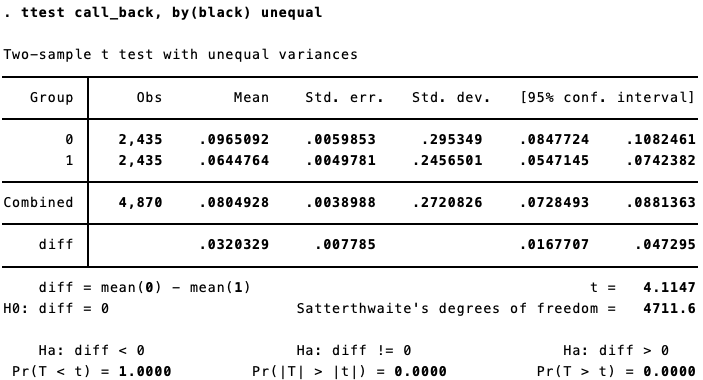
\includegraphics[width=0.85\linewidth]{pictures/res2-ttestBlack} \end{center}

\normalsize

\(\Rightarrow\) Same conclusion as the first approach.
\end{frame}

\begin{frame}{(d) Is there any evidence of nonrandom assignment of race
~to resumes?}
\protect\hypertarget{d-is-there-any-evidence-of-nonrandom-assignment-of-race-to-resumes}{}
\begin{itemize}
\tightlist
\item
  Idea: Is there statistically significant difference in other
  characteristics for two groups - black and white sounding names?
  \footnotesize \protect\hyperlink{RCTC}{(\textgreater\textgreater review)}
  \normalsize
\end{itemize}

\vspace{0.8mm}

\begin{itemize}
\tightlist
\item
  Use any approach in (a), calculate estimated means of other
  characteristics for these two groups and test whether the difference
  is statistically significant.
\end{itemize}

\vspace{0.8mm}

\begin{itemize}
\tightlist
\item
  There are only two significant differences in the mean values: the
  call-back rate (the outcome variable of interest) and computer skills
  (for which black-named resumes had a slightly higher fraction that
  white-named resumes).
\end{itemize}

\(\Rightarrow\) There is no evidence of non-random assignment.
\end{frame}

\begin{frame}{(d) Is there any evidence of nonrandom assignment of race
~to resumes?}
\protect\hypertarget{d-is-there-any-evidence-of-nonrandom-assignment-of-race-to-resumes-1}{}
\footnotesize

\begin{center}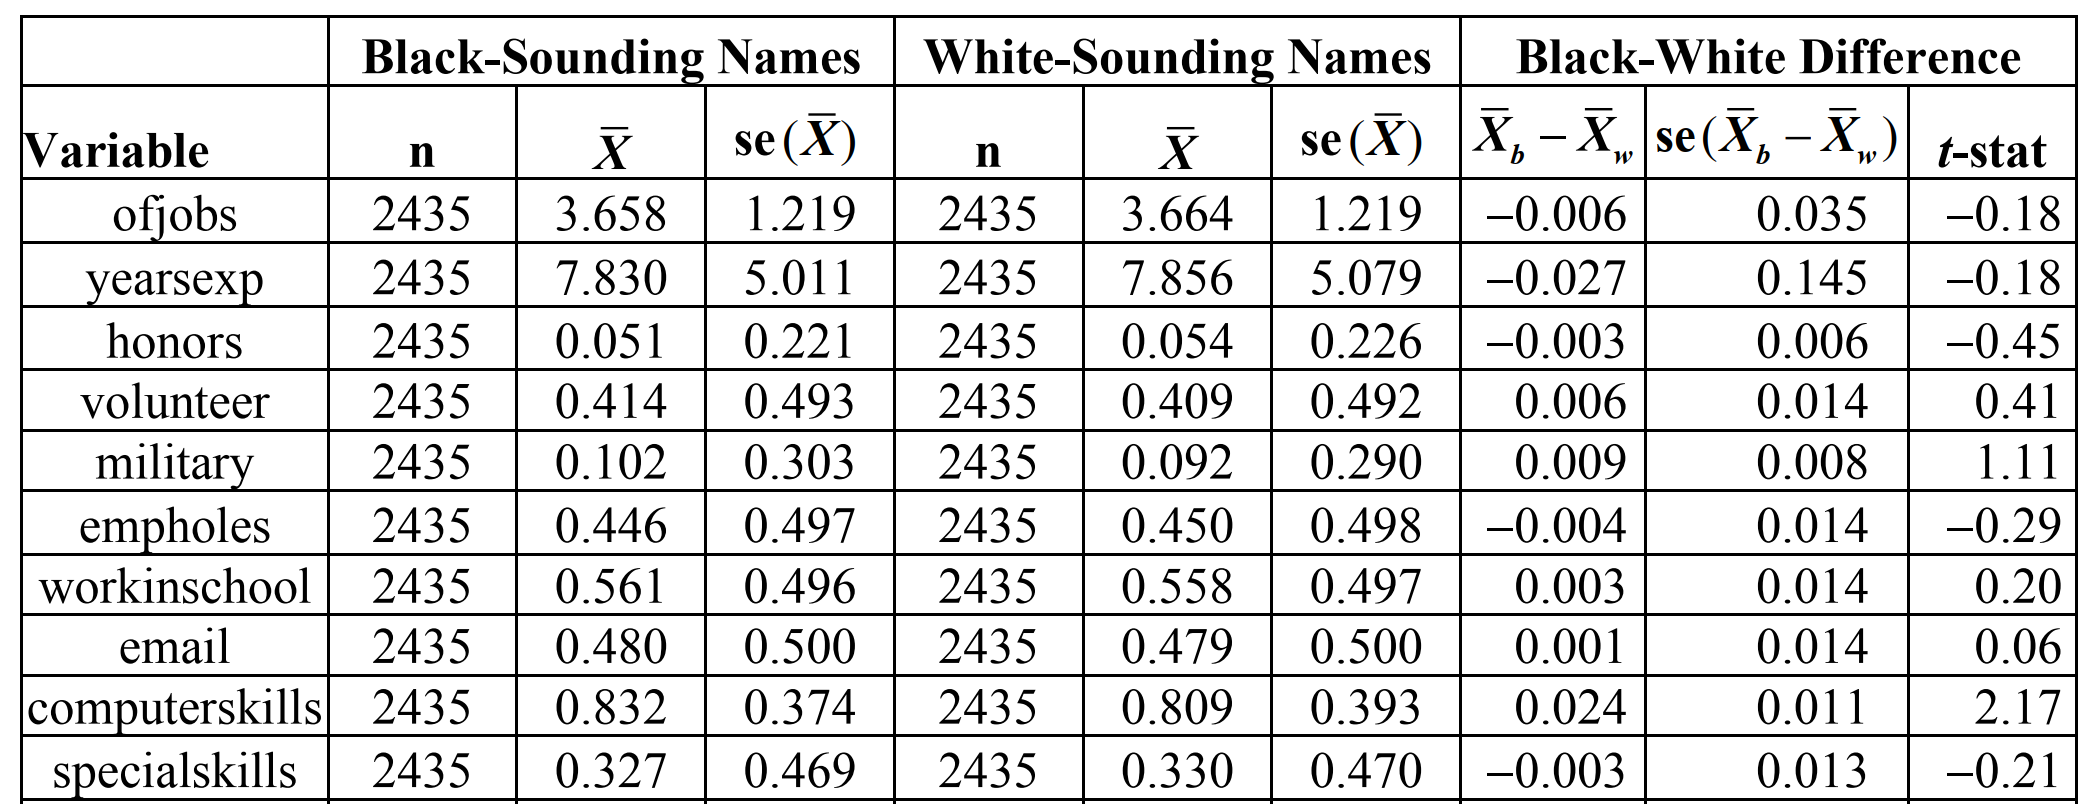
\includegraphics[width=1\linewidth]{pictures/otherW} \end{center}

\(\ldots\)
\end{frame}

\begin{frame}{(c1) Callback rates for high-quality versus low-quality
resumes?}
\protect\hypertarget{c1-callback-rates-for-high-quality-versus-low-quality-resumes}{}
\begin{itemize}
\item
  OLS estimation results
  \footnotesize \protect\hyperlink{res3-regHigh}{(\textgreater\textgreater stata)}
  \normalsize \[
  \begin{aligned}
  \underset{(se)}{\widehat{call\_back}} = \underset{(0.005)}{0.073} + \underset{(0.008)}{0.014}\cdot high
  \end{aligned}
  \]
\item
  On average, the call-back rate for low-quality resumes is \(0.073\)
  and for high-quality resumes is \(0.073 + 0.014 = 0.087\).
\item
  The difference is \(0.014\), which is not significant at the \(5\%\)
  level, but is at the \(10\%\) level (\(t-statistic = 1.80\))
\end{itemize}
\end{frame}

\begin{frame}{(c2) A significant difference in the
high-quality/low-quality difference for whites versus African
Americans?}
\protect\hypertarget{c2-a-significant-difference-in-the-high-qualitylow-quality-difference-for-whites-versus-african-americans}{}
\textbf{Model specification}

\[
call\_back_i = \beta_0 + \beta_1\cdot black_i + \beta_2 \cdot high_i + \beta_3 \cdot black_i \times high_i+ u_i
\] \small \[
\begin{aligned}
E[call\_back \mid high = 1, black = 1] &= \beta_0 + \beta_1 + \beta_2 + \beta_3 \rightarrow \text{for high-quality blacks}\\
E[call\_back \mid high = 0, black = 1] &= \beta_0 + \beta_1 \rightarrow \text{for low-quality blacks}\\
\Delta^{HvL}_{black = 1} &= \beta_2 + \beta_3 \rightarrow \text{the h/l difference in black group}\\
\\
E[call\_back \mid high = 1, black = 0] &= \beta_0 + \beta_2 \rightarrow \text{for high-quality whites}\\
E[call\_back \mid high = 0, black = 0] &= \beta_0 \rightarrow \text{for low-quality whites}\\
\Delta^{HvL}_{black = 0} &= \beta_2 \rightarrow \text{the h/l difference in white group}\\
\\
\Delta^{HvL}_{black = 1} - \Delta^{HvL}_{black = 0} &= \beta_3
\end{aligned}
\]
\end{frame}

\begin{frame}{(c2) A significant difference in the
high-quality/low-quality difference for whites versus African
Americans?}
\protect\hypertarget{c2-a-significant-difference-in-the-high-qualitylow-quality-difference-for-whites-versus-african-americans-1}{}
\begin{itemize}
\tightlist
\item
  OLS estimation results
  \footnotesize \protect\hyperlink{res4-regHighBlack}{(\textgreater\textgreater stata)}
  \normalsize \small \[
  \begin{aligned}
  \underset{(se)}{\widehat{call\_back}} = \underset{(0.008)}{0.084} - \underset{(0.011)}{0.023}\cdot black + \underset{(0.012)}{0.023}\cdot high - \underset{(0.016)}{0.018}\cdot black \times high
  \end{aligned}
  \]
\end{itemize}

\normalsize

\begin{itemize}
\tightlist
\item
  On average, the high-quality/low-quality difference for whites is
  \(\hat{\beta}_2 = 0.023\) and for blacks is
  \(\hat{\beta}_2 + \hat{\beta}_3 = 0.023 - 0.018 = 0.005\).
\end{itemize}

\vspace{0.8mm}

\begin{itemize}
\tightlist
\item
  The black-white difference is \(\hat{\beta}_3 = -0.018\), which is not
  statistically significant at the \(5\%\) level
  (\(t-statistic = -1.14\)).
\end{itemize}
\end{frame}

\begin{frame}{Table of Results}
\protect\hypertarget{table-of-results}{}
\small

\begin{table}[]
\centering
\begin{tabular}{@{}|l|ccc|@{}}
\toprule
 &
  \multicolumn{3}{l|}{\textbf{Dependent Variable = call$\_$back}} \\ \midrule
\textbf{Regressor} &
  \multicolumn{1}{c|}{\textbf{(a)}} &
  \multicolumn{1}{c|}{\textbf{(c1)}} &
  \textbf{(c2)} \\ \midrule
\textit{black} &
  \multicolumn{1}{c|}{\begin{tabular}[c]{@{}c@{}}-0.032\\ (0.008)\end{tabular}} &
  \multicolumn{1}{c|}{} &
  \begin{tabular}[c]{@{}c@{}}-0.023\\ (0.011)\end{tabular} \\ \midrule
\textit{high} &
  \multicolumn{1}{c|}{} &
  \multicolumn{1}{c|}{\begin{tabular}[c]{@{}c@{}}0.014\\ (0.008)\end{tabular}} &
  \begin{tabular}[c]{@{}c@{}}0.023\\ (0.012)\end{tabular} \\ \midrule
\textit{black $\times$ high} &
  \multicolumn{1}{c|}{} &
  \multicolumn{1}{c|}{} &
  \begin{tabular}[c]{@{}c@{}}-0.018\\ (0.016)\end{tabular} \\ \midrule
\textit{Intercept} &
  \multicolumn{1}{c|}{\begin{tabular}[c]{@{}c@{}}0.097\\ (0.006)\end{tabular}} &
  \multicolumn{1}{c|}{\begin{tabular}[c]{@{}c@{}}0.073\\ (0.005)\end{tabular}} &
  \begin{tabular}[c]{@{}c@{}}0.084\\ (0.008)\end{tabular} \\ \bottomrule
\end{tabular}
\end{table}

\center\footnotesize Notes: Standard errors shown in parentheses.
\end{frame}

\hypertarget{exercise-1-based-on-stock-and-watson-e8.1}{%
\section{Exercise 1: based on Stock and Watson,
E8.1}\label{exercise-1-based-on-stock-and-watson-e8.1}}

\begin{frame}[fragile]{Picture the Scenario}
\protect\hypertarget{picture-the-scenario-2}{}
\begin{itemize}
\tightlist
\item
  \textbf{Objective:} Investigate the effect of \emph{lead water pipes}
  on \emph{infant mortality} (\emph{with a focus on interaction
  effects}).
\end{itemize}

\vspace{0.8mm}

\begin{itemize}
\tightlist
\item
  \textbf{Dataset:} \texttt{lead$\_$mortality.dta}

  \begin{itemize}
  \tightlist
  \item
    Data for 172 U.S. cities in 1900.
  \end{itemize}
\end{itemize}

\vspace{0.8mm}

\begin{itemize}
\tightlist
\item
  \textbf{Key variables:}

  \begin{itemize}
  \tightlist
  \item
    \texttt{Lead}: type of water pipes (lead or nonlead).
  \item
    \texttt{Inf}: the average infant mortality rate.
  \item
    \texttt{pH}: water acidity.
  \item
    several demographic variables.
  \end{itemize}
\end{itemize}
\end{frame}

\begin{frame}[fragile]{Questions}
\protect\hypertarget{questions-2}{}
\begin{enumerate}
[(a)]
\tightlist
\item
  Compute the average infant mortality rate (\texttt{Inf}) for cities
  with lead pipes and for cities with nonlead pipes.\\
  Is there a statistically significant difference in the averages?
\end{enumerate}
\end{frame}

\begin{frame}[fragile]{Questions}
\protect\hypertarget{questions-3}{}
\begin{enumerate}
[(a)]
\setcounter{enumi}{1}
\tightlist
\item
  The amount of lead leached from lead pipes depends on the chemistry of
  the water running through the pipes. The more acidic the water is
  (i.e.~the lower its pH), the more lead is leached. Run a regression of
  \texttt{Inf} on \texttt{Lead}, \texttt{pH}, and the interaction term
  \texttt{Lead} \(\times\) \texttt{pH}. \small
\end{enumerate}

\begin{enumerate}
\item
  Explain what coefficients measure.
\item
  Plot the estimated regression function relating \texttt{Inf} to
  \texttt{pH} for \(Lead = 0\) and for \(Lead = 1\).
\item
  Does \texttt{Lead} have a statistically significant effect on
  \texttt{Inf}? Explain.
\item
  Does the effect of \texttt{Lead} on \texttt{Inf} depend on
  \texttt{pH}? Is this dependence statistically significant?
\item
  What is the median value of \texttt{pH} in the sample? At this
  \texttt{pH} level, what is the estimated effect of \texttt{Lead} on
  \texttt{Inf}? What is the standard deviation of \texttt{pH}?\\
  Suppose the pH level is one standard deviation lower than the median
  level of pH in the sample: What is the estimated effect of Lead on
  infant mortality?\\
  What if pH is one standard deviation higher than the median value?
\end{enumerate}
\end{frame}

\begin{frame}[fragile]{(a) Compute the average \texttt{Inf} for cities
with lead pipes and for cities with nonlead pipes. Is there a
statistically significant difference in the averages?}
\protect\hypertarget{a-compute-the-average-inf-for-cities-with-lead-pipes-and-for-cities-with-nonlead-pipes.-is-there-a-statistically-significant-difference-in-the-averages}{}
\textbf{Two-sample t test} \footnotesize

\begin{Shaded}
\begin{Highlighting}[]
\NormalTok{* }\KeywordTok{ttest}\NormalTok{ yvar, }\KeywordTok{by}\NormalTok{(groupvar) unequal}
\CommentTok{// Test if mean(yvar) equal between 2 groups defined by groupvar}
\CommentTok{// add option \textquotesingle{}unequal\textquotesingle{} to assume unequal variances}
\end{Highlighting}
\end{Shaded}
\end{frame}

\begin{frame}{(a) Compute the average \texttt{Inf} for cities with lead
pipes and for cities with nonlead pipes. Is there a statistically
significant difference in the averages?}
\protect\hypertarget{a-compute-the-average-inf-for-cities-with-lead-pipes-and-for-cities-with-nonlead-pipes.-is-there-a-statistically-significant-difference-in-the-averages-1}{}
\footnotesize

\begin{center}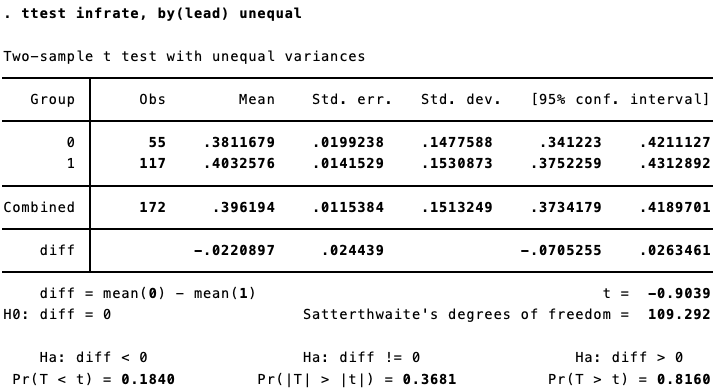
\includegraphics[width=1\linewidth]{pictures/ex1-res1-ttestLead} \end{center}
\end{frame}

\begin{frame}{(a) Compute the average \texttt{Inf} for cities with lead
pipes and for cities with nonlead pipes. Is there a statistically
significant difference in the averages?}
\protect\hypertarget{a-compute-the-average-inf-for-cities-with-lead-pipes-and-for-cities-with-nonlead-pipes.-is-there-a-statistically-significant-difference-in-the-averages-2}{}
\begin{table}[]
\centering
\begin{tabular}{|l|r|r|r|}
\hline
                             & n & $\bar{Y}$ & SE($\bar{Y}$) \\ \hline
Lead    & 117 & 0.403 & 0.014 \\ \hline
No Lead & 55  & 0.381 & 0.020 \\ \hline
\textit{Difference} &            & \textit{0.022}                    & \textit{0.024}                        \\ \hline
\end{tabular}
\end{table}

\small

\begin{itemize}
\item
  The difference in the sample means is 0.022 with a standard error of
  0.024. \vspace{0.8mm}
\item
  The estimate implies that cities with lead pipes have a larger infant
  mortality rate (by 0.02 deaths per 100 people in the population), but
  the standard error is large (0.024) and the difference is not
  statistically significant (\(t = 0.022/0.024 \approx 0.9\)).
\end{itemize}
\end{frame}

\begin{frame}{(b) Regression of \texttt{Inf} on \texttt{Lead},
\texttt{pH}, and the interaction ~~term \texttt{Lead} \(\times\)
\texttt{pH}}
\protect\hypertarget{b-regression-of-inf-on-lead-ph-and-the-interaction-term-lead-times-ph}{}
\textbf{Model specification}

\[
Inf_i = \beta_0 + \beta_1\cdot Lead_i + \beta_2 \cdot pH_i + \beta_3 \cdot Lead_i \times pH_i + u_i
\]

\[
\begin{aligned}
(1)\quad \color{blue}{E[Inf \mid Lead, pH]} &\color{blue}{= \beta_0 + (\beta_1 \cdot Lead + \beta_2 \cdot pH + \beta_3 \cdot pH \times Lead)}\\
\\
(2)\quad \color{red}{E[Inf \mid Lead, pH]} &\color{red}{= (\beta_0 + \beta_2 \cdot pH) + (\beta_1 + \beta_3 \cdot pH) \times Lead}\\
\\
(3)\quad \color{green}{E[Inf \mid Lead, pH]} &\color{green}{= (\beta_0 + \beta_1 \cdot Lead) + (\beta_2 + \beta_3 \cdot Lead) \times pH}
\end{aligned}
\]
\end{frame}

\begin{frame}[fragile]{(b1) Understand what coefficients measure.}
\protect\hypertarget{b1-understand-what-coefficients-measure.}{}
\[
\begin{aligned}
\text{From (1):} \quad  \color{blue}{E[Inf \mid Lead, pH]} &\color{blue}{= \beta_0 + (\beta_1 \cdot Lead + \beta_2 \cdot pH + \beta_3 \cdot pH \times Lead)}\\
\\
E[Inf \mid Lead = 0, pH = 0] &= \beta_0\\
\end{aligned}
\]

\(\Rightarrow\) The intercept \(\beta_0\) shows the level of
\texttt{Inf} when \(Lead = 0\) and \(pH = 0\). It dictates the level of
the regression line.
\end{frame}

\begin{frame}[fragile]{(b1) Understand what coefficients measure.}
\protect\hypertarget{b1-understand-what-coefficients-measure.-1}{}
\[
\begin{aligned}
\text{From (2):} \quad \color{red}{E[Inf \mid Lead, pH]} &\color{red}{= (\beta_0 + \beta_2 \cdot pH) + (\beta_1 + \beta_3 \cdot pH) \times Lead}\\
\\
E[Inf \mid Lead = 1, pH] &= (\beta_0 + \beta_2 \cdot pH) + (\beta_1 + \beta_3 \cdot pH)\\
E[Inf \mid Lead = 0, pH] &= (\beta_0 + \beta_2 \cdot pH)\\
\rightarrow \Delta^{Lead-NoLead}_{pH \text{ fixed}} &= \hspace{2.6cm} (\beta_1 + \beta_3 \cdot pH)
\end{aligned}
\]

\(\Rightarrow\) \(\beta_1\) and \(\beta_3\) measure the effect of
\texttt{Lead} on \texttt{Inf}. Comparing 2 cities, one with lead pipes
(\(Lead = 1\)) and one without lead pipes (\(Lead = 0\)), but the same
of \texttt{pH}, the difference in infant mortality rate on average is
\(\beta_1 + \beta_3 \cdot pH\).
\end{frame}

\begin{frame}[fragile]{(b1) Understand what coefficients measure.}
\protect\hypertarget{b1-understand-what-coefficients-measure.-2}{}
\[
\begin{aligned}
\text{From (3):} \quad \color{green}{E[Inf \mid Lead, pH]} &\color{green}{= (\beta_0 + \beta_1 \cdot Lead) + (\beta_2 + \beta_3 \cdot Lead) \times pH}\\
\\
E[Inf \mid pH = c+1, Lead] &=(\beta_0 + \beta_1 \cdot Lead) + (\beta_2 + \beta_3 \cdot Lead) \times (c + 1)\\
E[Inf \mid pH = c, Lead] &= (\beta_0 + \beta_1 \cdot Lead) + (\beta_2 + \beta_3 \cdot Lead) \times c\\
\rightarrow \Delta^{\text{increase pH by 1}}_{Lead \text{ fixed}} &= \hspace{2.85cm}(\beta_2 + \beta_3 \cdot Lead)
\end{aligned}
\]

\(\Rightarrow\) \(\beta_2\) and \(\beta_3\) measure the effect of
\texttt{pH} on \texttt{Inf}. Comparing 2 cities, with 1 unit
differential in \texttt{pH}, but the same of \texttt{Lead}, the
difference in infant mortality rate on average is
\(\beta_2 + \beta_3 \cdot Lead\).
\end{frame}

\begin{frame}[fragile]{(b1) Run the regression and Interpret.}
\protect\hypertarget{b1-run-the-regression-and-interpret.}{}
OLS estimation results
\footnotesize \protect\hyperlink{ux5cux23ex1-res2-regLeadpH}{(\textgreater\textgreater stata)}
\normalsize \[
\underset{(se)}{\widehat{Inf}} = \underset{(0.150)}{0.919} + \underset{(0.208)}{0.462} \cdot Lead - \underset{(0.021)}{0.075} \cdot pH - \underset{(0.028)}{0.057} \cdot Lead \times pH
\]

\small

\pause

\begin{itemize}
\tightlist
\item
  \(\hat{\beta}_0 = 0.919\) shows the level of \texttt{Inf} when
  \(Lead = 0\) and \(pH = 0\). It dictates the level of the regression
  line.
\end{itemize}

\pause

\begin{itemize}
\item
  Comparing 2 cities, one with lead pipes \(Lead = 0\) and one without
  lead pipes \(Lead = 0\), but the same of pH, the difference in
  predicted infant mortality rate is \[
  (2') \quad \widehat{Inf}(Lead=1,pH) - \widehat{Inf}(Lead=0,pH) = 0.462-0.057\cdot pH 
  \] \pause
\item
  Comparing 2 cities, one with \(pH = 6\) and one with with \(pH = 6\),
  but the same of \texttt{Lead}, the difference in predicted infant
  mortality rate is \[
  (3') \quad \widehat{Inf}(pH = 6,Lead) - \widehat{Inf}(pH = 5,Lead) = -0.075-0.057\cdot Lead 
  \] \(\Rightarrow\) so the difference is \(-0.075\) for cities without
  lead pipes and \(-0.132\) for cities with lead pipes.
\end{itemize}
\end{frame}

\begin{frame}{(b2) Plot the estimated regression function relating
\texttt{Inf} to \texttt{pH} for \(Lead = 0\) and for \(Lead = 1\).}
\protect\hypertarget{b2-plot-the-estimated-regression-function-relating-inf-to-ph-for-lead-0-and-for-lead-1.}{}
\begin{center}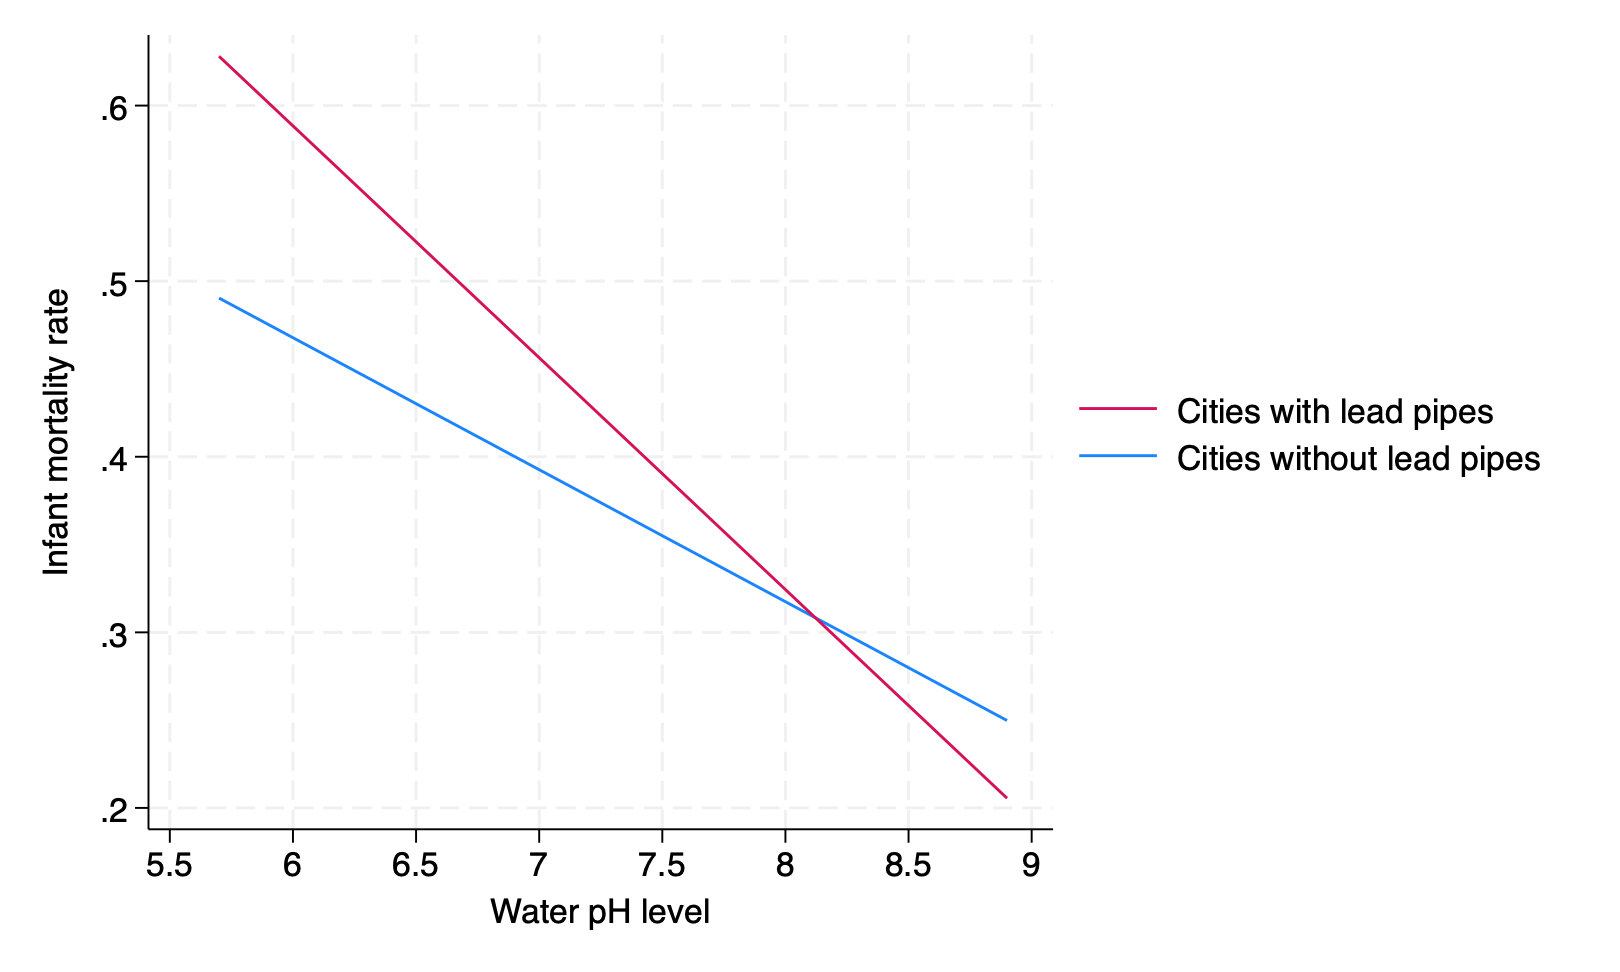
\includegraphics[width=0.8\linewidth]{pictures/ex1-Lineplot} \end{center}

\(\Rightarrow\) The infant mortality rate is higher for cities with lead
pipes, but the difference declines as the pH level increases.
\footnotesize \protect\hyperlink{ex1-res3-plotRegLine}{(\textgreater\textgreater stata)}
\normalsize
\end{frame}

\begin{frame}{(b2) The difference in infant mortality rates between
cities with lead pipes and cites without lead pipes}
\protect\hypertarget{b2-the-difference-in-infant-mortality-rates-between-cities-with-lead-pipes-and-cites-without-lead-pipes}{}
\normalsize

\begin{itemize}
\tightlist
\item
  At the \(10^{th}\) percentile of pH (\(6.4\)) is \small \[
  \widehat{Inf}(Lead=1,pH=6.4) - \widehat{Inf}(Lead=0,pH=6.4) = 0.462-0.057\times6.4 \approx 0.097
  \] \normalsize
\item
  At the \(50^{th}\) percentile of pH (\(7.5\)) is \small \[
  \widehat{Inf}(Lead=1,pH=7.5) - \widehat{Inf}(Lead=0,pH=7.5) = 0.462-0.057\times7.5 \approx 0.035
  \] \normalsize
\item
  At the \(90^{th}\) percentile of pH (\(8.2\)) is \small \[
  \widehat{Inf}(Lead=1,pH=8.2) - \widehat{Inf}(Lead=0,pH=8.2) = 0.462-0.057\times8.2 \approx  0.005
  \]
\end{itemize}

\footnotesize

\begin{itemize}
\tightlist
\item
  \emph{Note: Refer to equation (2') in (b1).}
\end{itemize}
\end{frame}

\begin{frame}[fragile]{(b3) Does \texttt{Lead} have a statistically
significant effect on ~~\texttt{Inf}? Explain.}
\protect\hypertarget{b3-does-lead-have-a-statistically-significant-effect-on-inf-explain.}{}
\begin{itemize}
\tightlist
\item
  Null Hypothesis: \(H_0: \beta_1 = \beta_3 = 0\)
  \footnotesize \protect\hyperlink{ex1-res4-FtestLead}{(\textgreater\textgreater stata)}
  \normalsize
\end{itemize}

\vspace{0.8mm}

\begin{itemize}
\tightlist
\item
  The F-statistic for the coefficient on \texttt{Lead} and the
  interaction term is \(F = 3.94\), which has a p-value of 0.02, so the
  coefficients are jointly statistically significantly different from
  zero at the \(5\%\) but not the \(1\%\) significance level.
\end{itemize}
\end{frame}

\begin{frame}{(b4) Does the effect of \texttt{Lead} on \texttt{Inf}
depend on \texttt{pH}? Is this dependence statistically significant?}
\protect\hypertarget{b4-does-the-effect-of-lead-on-inf-depend-on-ph-is-this-dependence-statistically-significant}{}
\begin{itemize}
\tightlist
\item
  Null Hypothesis: \(H_0: \beta_3 = 0\)
  \footnotesize \protect\hyperlink{ux5cux23ex1-res2-regLeadpH}{(\textgreater\textgreater stata)}
  \normalsize
\end{itemize}

\vspace{0.8mm}

\begin{itemize}
\tightlist
\item
  The interaction term has a t statistic of \(t = -2.02\), so the
  coefficient is significant at the \(5\%\) but not the \(1\%\)
  significance level.
\end{itemize}
\end{frame}

\hypertarget{brief-review}{%
\section{BRIEF REVIEW}\label{brief-review}}

\begin{frame}{Causal Graph (I)}
\protect\hypertarget{RCT}{}
\begin{block}{Randomized Experiment}
\protect\hypertarget{randomized-experiment}{}
\begin{center}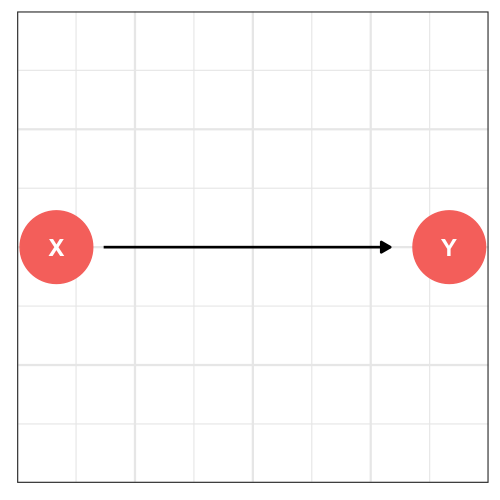
\includegraphics[width=0.4\linewidth,height=0.54\textheight]{pictures/RCTsetting1} 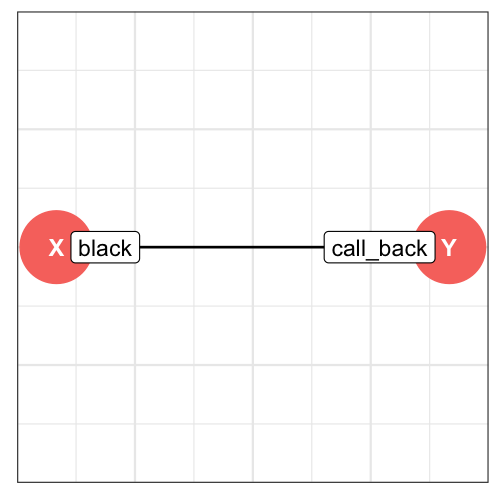
\includegraphics[width=0.4\linewidth,height=0.54\textheight]{pictures/RCTsetting2} \end{center}

\footnotesize\protect\hyperlink{RCTQ}{(\textgreater\textgreater back)}
\normalsize
\end{block}
\end{frame}

\begin{frame}{Causal Graph (II)}
\protect\hypertarget{RCTC}{}
\begin{block}{Randomized Experiment with additional characteristics}
\protect\hypertarget{randomized-experiment-with-additional-characteristics}{}
\begin{center}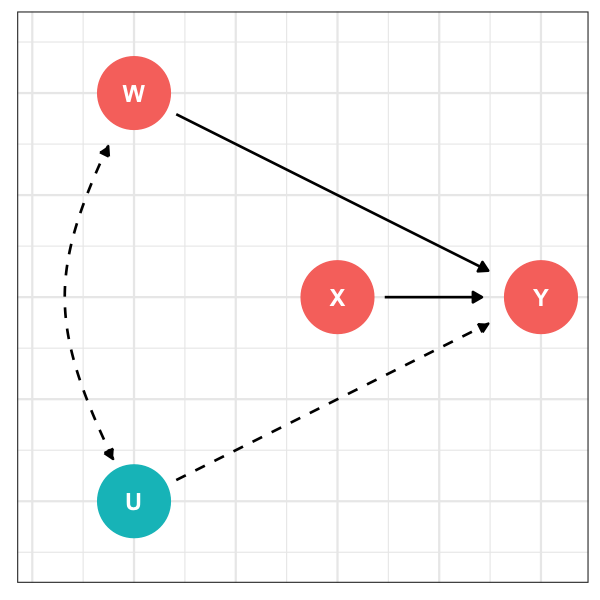
\includegraphics[width=0.4\linewidth,height=0.54\textheight]{pictures/RCTCsetting1} 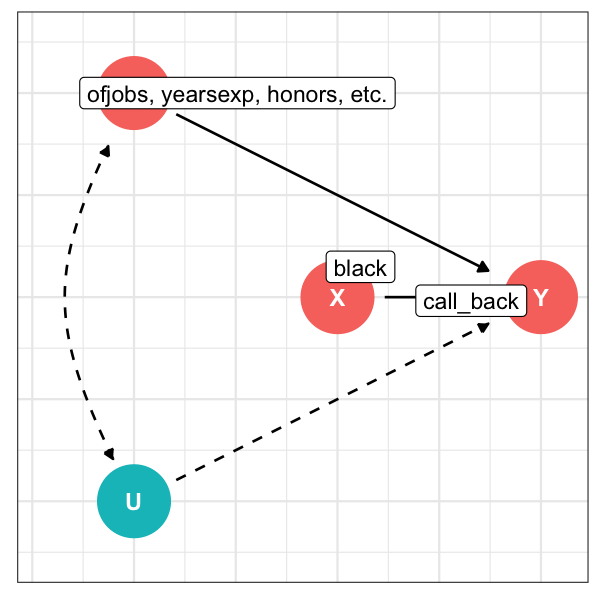
\includegraphics[width=0.4\linewidth,height=0.54\textheight]{pictures/RCTCsetting2} \end{center}

\footnotesize\protect\hyperlink{RCTQ}{(\textgreater\textgreater back)}
\normalsize
\end{block}
\end{frame}

\hypertarget{stata-codes-results}{%
\section{STATA CODES \& RESULTS}\label{stata-codes-results}}

\begin{frame}{Exercise 2(a)}
\protect\hypertarget{res1-regBlack}{}
\begin{center}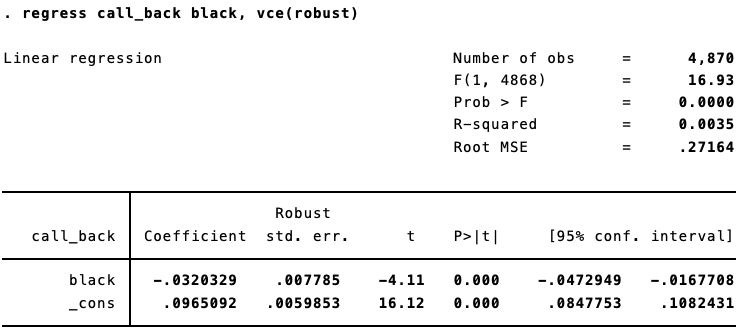
\includegraphics[width=1\linewidth]{pictures/res1-regBlack} \end{center}
\end{frame}

\begin{frame}[fragile]{Exercise 2(a)}
\protect\hypertarget{exercise-2a}{}
\small

\begin{Shaded}
\begin{Highlighting}[]
\NormalTok{* }\KeywordTok{ttest}\NormalTok{ yvar, }\KeywordTok{by}\NormalTok{(groupvar) unequal}
\CommentTok{// Test if mean(yvar) equal between 2 groups defined by groupvar}
\CommentTok{// add option \textquotesingle{}unequal\textquotesingle{} to assume unequal variances}
\end{Highlighting}
\end{Shaded}

\begin{center}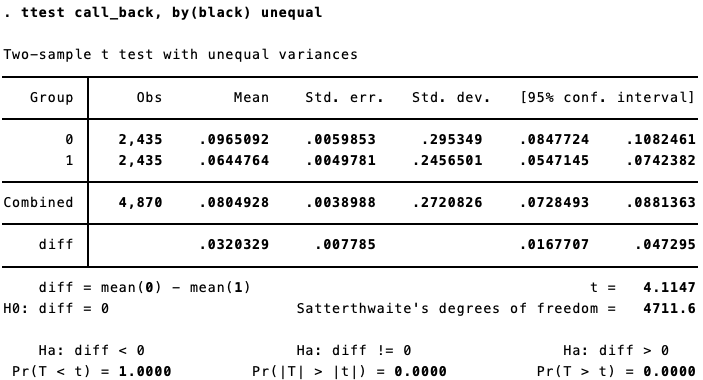
\includegraphics[width=0.9\linewidth]{pictures/res2-ttestBlack} \end{center}
\end{frame}

\begin{frame}{Exercise 2(c1)}
\protect\hypertarget{res3-regHigh}{}
\begin{center}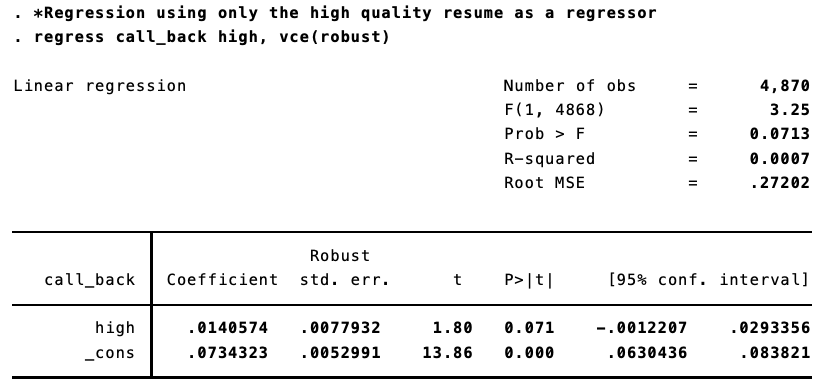
\includegraphics[width=1\linewidth]{pictures/res3-regHigh} \end{center}
\end{frame}

\begin{frame}{Exercise 2(c2)}
\protect\hypertarget{res4-regHighBlack}{}
\begin{center}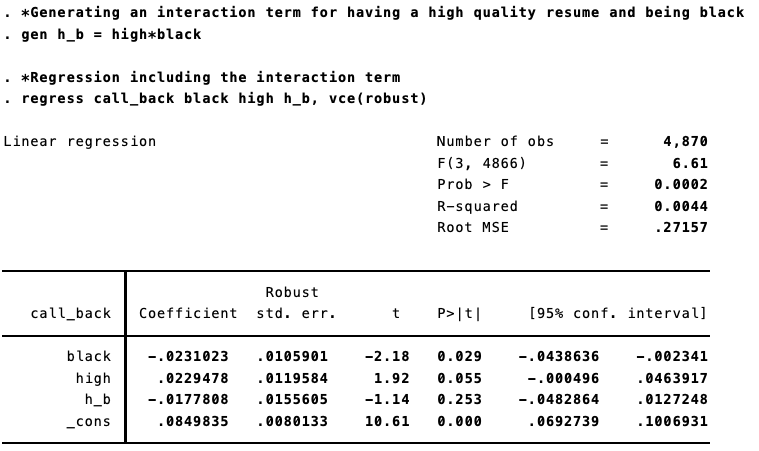
\includegraphics[width=1\linewidth]{pictures/res4-regHighBlack} \end{center}
\end{frame}

\begin{frame}{Exercise 1(a)}
\protect\hypertarget{ex1-res1-ttestLead}{}
\begin{center}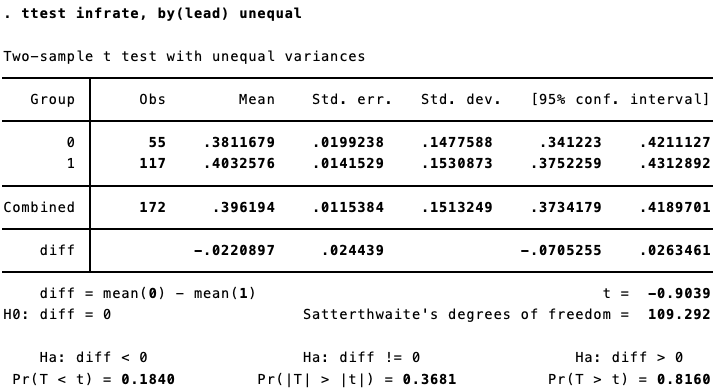
\includegraphics[width=1\linewidth]{pictures/ex1-res1-ttestLead} \end{center}
\end{frame}

\begin{frame}{Exercise 1(b1)}
\protect\hypertarget{ex1-res2-regLeadpH}{}
\begin{center}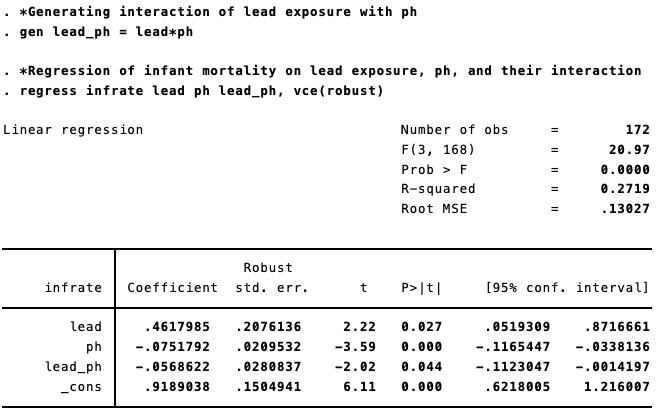
\includegraphics[width=1\linewidth]{pictures/ex1-res2-regLeadpH} \end{center}
\end{frame}

\begin{frame}{Exercise 1(b2)}
\protect\hypertarget{ex1-res3-plotRegLine}{}
\begin{center}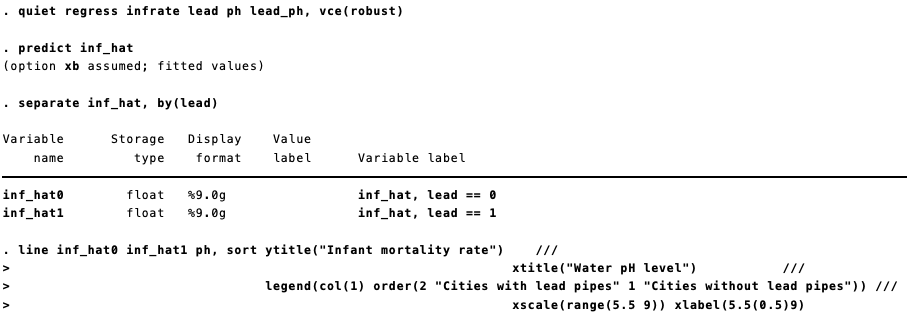
\includegraphics[width=1\linewidth]{pictures/ex1-res3-plotRegLine} \end{center}
\end{frame}

\begin{frame}{Exercise 1(b3)}
\protect\hypertarget{ex1-res4-FtestLead}{}
\begin{center}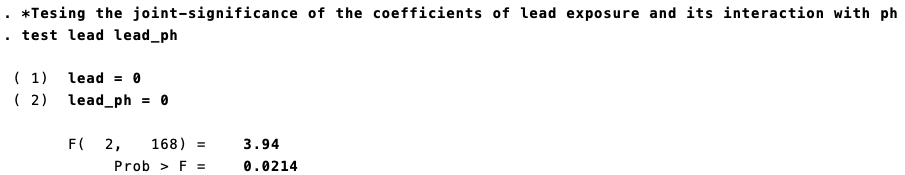
\includegraphics[width=1\linewidth]{pictures/ex1-res4-FtestLead} \end{center}
\end{frame}

\end{document}
